\documentclass[aspectratio=169]{beamer}
\usepackage{graphicx}
\usepackage{tikz}
\usetikzlibrary{shapes.geometric, arrows.meta, positioning, fit, backgrounds, calc}
\usepackage{booktabs}
\usepackage{pifont}

% Custom restrained academic palette
\definecolor{navy}{RGB}{20, 30, 60}
\definecolor{charcoal}{RGB}{50, 50, 50}
\definecolor{accent}{RGB}{0, 102, 204}
\definecolor{errorred}{RGB}{200, 40, 40}
\definecolor{successgreen}{RGB}{40, 140, 60}

\usetheme{default}
\usefonttheme{default}
\setbeamercolor{structure}{fg=navy}
\setbeamercolor{title}{fg=navy}
\setbeamercolor{frametitle}{fg=navy, bg=white}
\setbeamercolor{normal text}{fg=charcoal}
\setbeamercolor{itemize item}{fg=accent}
\setbeamertemplate{navigation symbols}{}
\setbeamertemplate{footline}[frame number]
\setbeamertemplate{frametitle}{\vspace{0.3cm}\Large\bfseries\insertframetitle}

\begin{document}

% SLIDE 1: Title
\begin{frame}[plain]
    \begin{center}
        \vspace{0.1cm}
        \IfFileExists{vu_logo.png}{
\includegraphics[width=0.7in]{vu_logo.png}\\[0.1cm]}{}
        {\Large \bfseries \textcolor{navy}{Signal-Aware ML Calibration for\\[0.1cm] Low-Cost Pan-Tilt LiDAR}} \\[0.2cm]
        {\normalsize Undergraduate Thesis Proposal} \\[0.1cm]
        {\footnotesize CSE 4100: Project or Thesis with Seminar Part I} \\[0.3cm]
        
        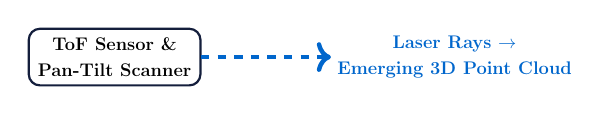
\begin{tikzpicture}[scale=0.55, transform shape]
            \node[draw=navy, thick, rounded corners, inner sep=6pt, align=center, font=\large\bfseries] (sensor) {ToF Sensor \&\\[0.1cm]Pan-Tilt Scanner};
            \draw[->, accent, ultra thick, dashed] (sensor.east) -- ++(3,0) node[right, align=center, font=\large\bfseries] {Laser Rays $\rightarrow$ \\[0.1cm] Emerging 3D Point Cloud};
        \end{tikzpicture}\\[0.3cm]

        {\scriptsize 
        \textbf{Students:} Abdul Momit Talukder (232311320) | Oishi Farzana (232311294) | Mahfuz Ahmad (232311307) \\[0.1cm]
        \textbf{Supervisor:} Mohd Ruhul Ameen, Lecturer \\[0.1cm]
        Department of Computer Science and Engineering | Varendra University
        }
    \end{center}
\end{frame}

% SLIDE 2: How Do Machines See 3D?
\begin{frame}{How Do Machines ``See'' 3D?}
    \begin{center}
        \vspace{0.5cm}
        {\Huge \textbf{\textcolor{navy}{Distance + Direction $\rightarrow$ 3D Geometry}}}
        
        \vspace{1.5cm}
        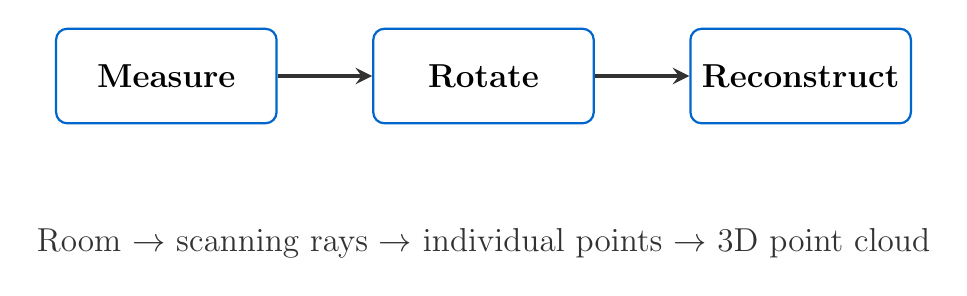
\begin{tikzpicture}[
            box/.style={draw=accent, thick, rounded corners, minimum width=2.8cm, minimum height=1.2cm, align=center, font=\large\bfseries},
            arrow/.style={->, >=stealth, ultra thick, charcoal}
        ]
            \node[box] (measure) {Measure};
            \node[box, right=1.2cm of measure] (rotate) {Rotate};
            \node[box, right=1.2cm of rotate] (reconstruct) {Reconstruct};
            
            \draw[arrow] (measure) -- (rotate);
            \draw[arrow] (rotate) -- (reconstruct);
            
            \node[below=1.2cm of rotate, text=charcoal, font=\large] (room) {Room $\rightarrow$ scanning rays $\rightarrow$ individual points $\rightarrow$ 3D point cloud};
        \end{tikzpicture}
    \end{center}
\end{frame}

% SLIDE 3: Motivation
\begin{frame}{3D Sensing Is Powerful — But Expensive}
    \vspace{0.5cm}
    \begin{columns}
        \column{0.5\textwidth}
        \begin{center}
            {\Huge \bfseries \textcolor{errorred}{\$500+}} \\[0.5cm]
            {\Large Commercial LiDAR}
        \end{center}
        \column{0.5\textwidth}
        \begin{center}
            {\Huge \bfseries \textcolor{successgreen}{$\sim$\$25}} \\[0.5cm]
            {\Large Our Target}
        \end{center}
    \end{columns}
    \vspace{1.5cm}
    \begin{center}
        {\Large \bfseries High performance is expensive. \\[0.2cm]
        Low cost often means lower accuracy.}
    \end{center}
\end{frame}

% SLIDE 4: Why Time of Flight
\begin{frame}{Why Time-of-Flight?}
    \vspace{0.5cm}
    \begin{columns}[t]
        \column{0.33\textwidth}
        \begin{center}
            \IfFileExists{figures/slide4_img0.png}{
\includegraphics[height=1.2cm, keepaspectratio]{figures/slide4_img0.png}\\[0.3cm]}{}
            {\large \bfseries Ultrasonic} \\[0.3cm]
            \textcolor{errorred}{\ding{55}} Wide beam \\[0.1cm]
            \textcolor{errorred}{\ding{55}} Lower spatial resolution
        \end{center}
        \column{0.33\textwidth}
        \begin{center}
            \IfFileExists{figures/slide4_img1.png}{
\includegraphics[height=1.2cm, keepaspectratio]{figures/slide4_img1.png}\\[0.3cm]}{}
            {\large \bfseries Radar} \\[0.3cm]
            \textcolor{errorred}{\ding{55}} Strong indoor complexity
        \end{center}
        \column{0.33\textwidth}
        \begin{center}
            \IfFileExists{figures/slide4_img2.png}{
\includegraphics[height=1.2cm, keepaspectratio]{figures/slide4_img2.png}\\[0.3cm]}{}
            {\large \bfseries \textcolor{accent}{Time-of-Flight}} \\[0.3cm]
            \textcolor{successgreen}{\ding{51}} Compact \& Fast \\[0.1cm]
            \textcolor{successgreen}{\ding{51}} Fine spatial sensing
        \end{center}
    \end{columns}
\end{frame}

% SLIDE 5: Literature Review
\begin{frame}{Literature Review \& Research Gap}
    \vspace{0.1cm}
    \begin{itemize}
        \item \textbf{ToF Error:} Corti et al. and Frangez et al. highlight multipath interference.
        \item \textbf{ML Depth Correction:} Su et al. map complex ToF distortions using high-end GPUs.
        \item \textbf{Low-Cost Scanners:} Jimenez et al. built pan-tilt ToF systems, but lacked ML calibration.
    \end{itemize}
    \vspace{0.3cm}
    \begin{center}
        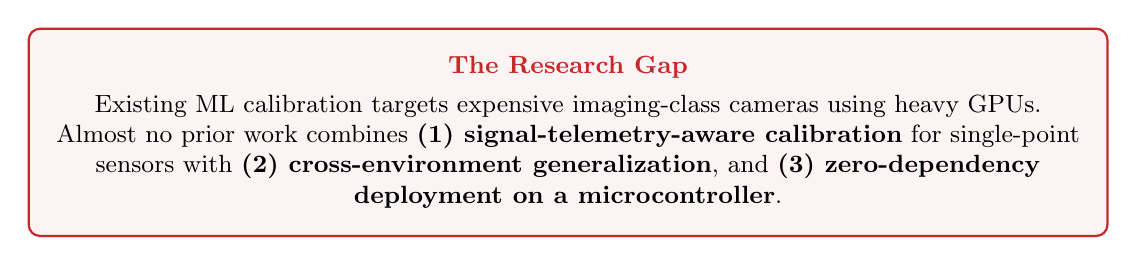
\begin{tikzpicture}
            \node[draw=errorred, thick, fill=errorred!5, rounded corners, inner sep=10pt, align=center, font=\small] {
                \textbf{\textcolor{errorred}{The Research Gap}} \\[0.1cm]
                Existing ML calibration targets expensive imaging-class cameras using heavy GPUs. \\
                Almost no prior work combines \textbf{(1) signal-telemetry-aware calibration} for single-point \\
                sensors with \textbf{(2) cross-environment generalization}, and \textbf{(3) zero-dependency} \\
                \textbf{deployment on a microcontroller}.
            };
        \end{tikzpicture}
    \end{center}
\end{frame}

% SLIDE 6: Objectives
\begin{frame}{Research Objectives}
    \vspace{0.5cm}
    \begin{center}
        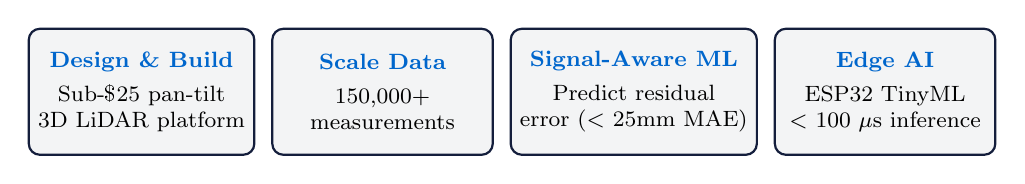
\begin{tikzpicture}[
            box/.style={draw=navy, thick, fill=navy!5, rounded corners, minimum width=2.8cm, minimum height=1.6cm, align=center, font=\footnotesize}
        ]
            \node[box] (obj1) {\textbf{\textcolor{accent}{Design \& Build}} \\[0.1cm] Sub-\$25 pan-tilt \\ 3D LiDAR platform};
            \node[box, right=0.2cm of obj1] (obj2) {\textbf{\textcolor{accent}{Scale Data}} \\[0.1cm] 150,000+ \\ measurements};
            \node[box, right=0.2cm of obj2] (obj3) {\textbf{\textcolor{accent}{Signal-Aware ML}} \\[0.1cm] Predict residual \\ error ($<$ 25mm MAE)};
            \node[box, right=0.2cm of obj3] (obj4) {\textbf{\textcolor{accent}{Edge AI}} \\[0.1cm] ESP32 TinyML \\ $<$ 100 $\mu$s inference};
        \end{tikzpicture}
    \end{center}
\end{frame}

% SLIDE 7: Hardware Architecture
\begin{frame}{Our Hardware Architecture}
    \begin{center}
        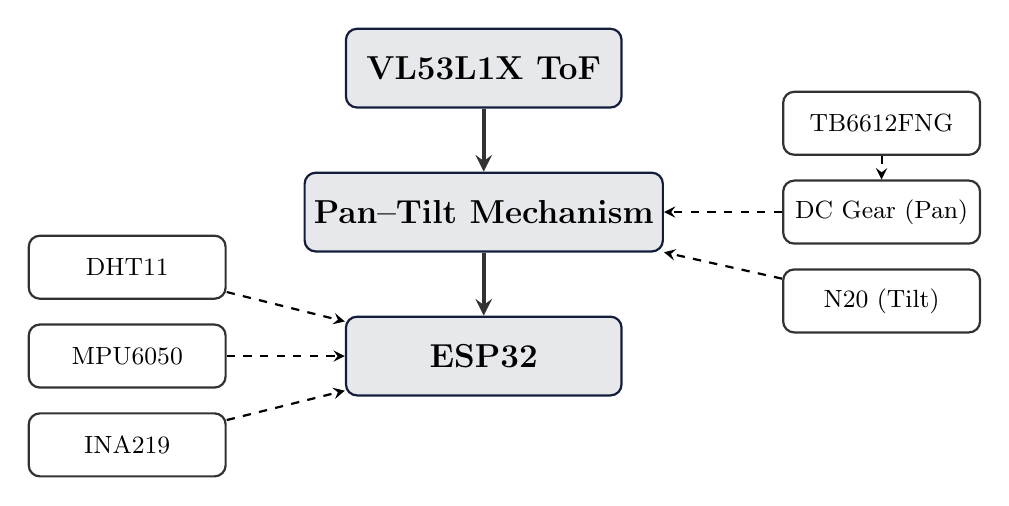
\begin{tikzpicture}[
            node distance=0.8cm and 1.5cm,
            mainbox/.style={draw=navy, thick, fill=navy!10, rounded corners, minimum width=3.5cm, minimum height=1cm, align=center, font=\large\bfseries},
            subbox/.style={draw=charcoal, thick, rounded corners, minimum width=2.5cm, minimum height=0.8cm, align=center, font=\small},
            arrow/.style={->, >=stealth, ultra thick, charcoal}
        ]
            \node[mainbox] (sensor) {VL53L1X ToF};
            \node[mainbox, below=0.8cm of sensor] (pantilt) {Pan--Tilt Mechanism};
            \node[mainbox, below=0.8cm of pantilt] (esp) {ESP32};
            
            \draw[arrow] (sensor) -- (pantilt);
            \draw[arrow] (pantilt) -- (esp);
            
            \node[subbox, left=of esp] (mpu) {MPU6050};
            \node[subbox, above=0.3cm of mpu] (dht) {DHT11};
            \node[subbox, below=0.3cm of mpu] (ina) {INA219};
            
            \draw[->, >=stealth, thick, dashed] (mpu) -- (esp);
            \draw[->, >=stealth, thick, dashed] (dht) -- (esp);
            \draw[->, >=stealth, thick, dashed] (ina) -- (esp);
            
            \node[subbox, right=of pantilt] (dc) {DC Gear (Pan)};
            \node[subbox, above=0.3cm of dc] (driver) {TB6612FNG};
            \node[subbox, below=0.3cm of dc] (n20) {N20 (Tilt)};
            
            \draw[->, >=stealth, thick, dashed] (dc) -- (pantilt);
            \draw[->, >=stealth, thick, dashed] (n20) -- (pantilt);
            \draw[->, >=stealth, thick, dashed] (driver) -- (dc);
        \end{tikzpicture}
    \end{center}
\end{frame}

% SLIDE 8: Concept to Pilot
\begin{frame}{From Concept to Pilot}
    \vspace{0.5cm}
    \begin{columns}
        \column{0.5\textwidth}
        \begin{center}
            \IfFileExists{figures/slide6_img0.png}{
                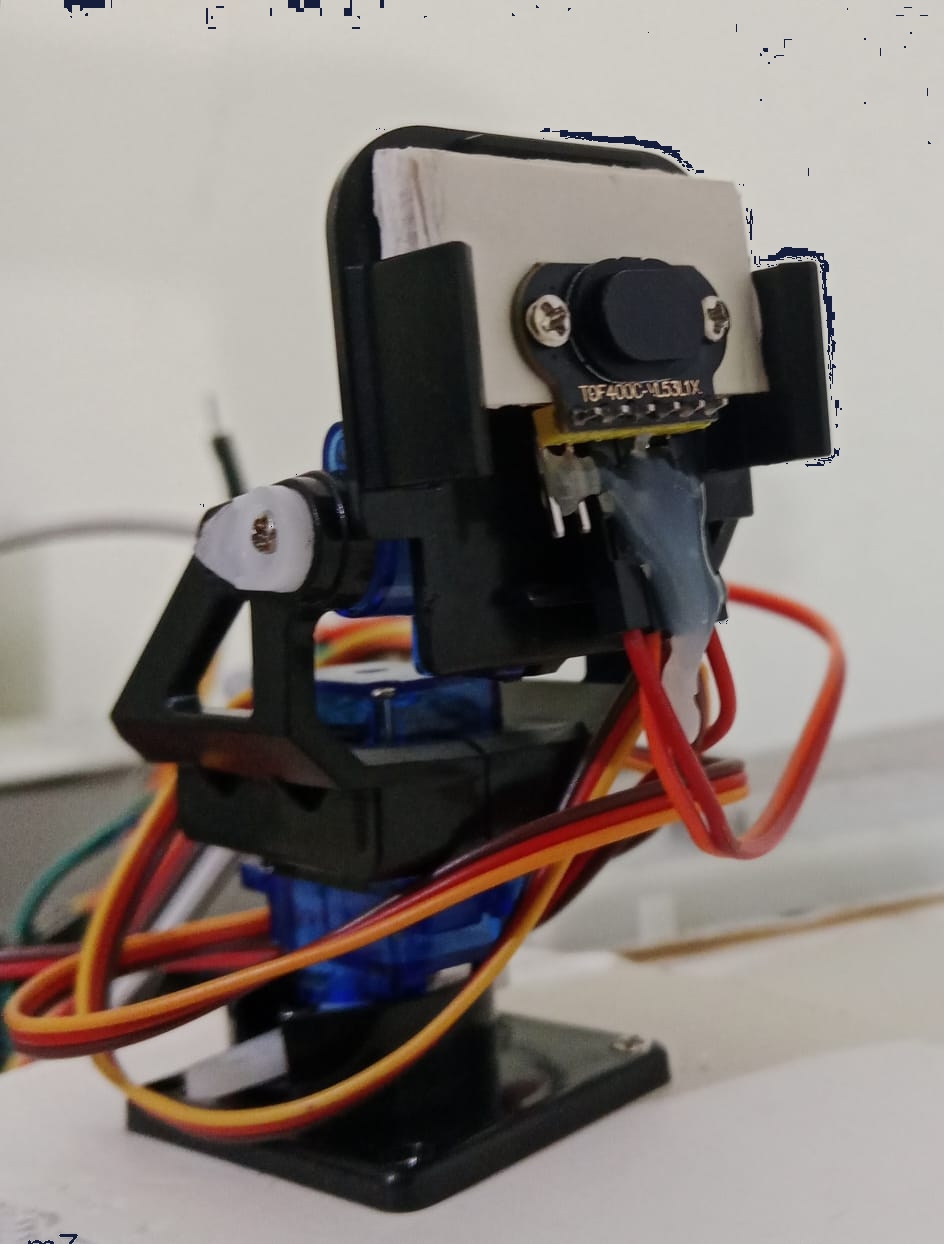
\includegraphics[height=4cm, keepaspectratio]{figures/slide6_img0.png} \\[0.2cm]
            }{
                \IfFileExists{figures/hardware_setup.png}{
                    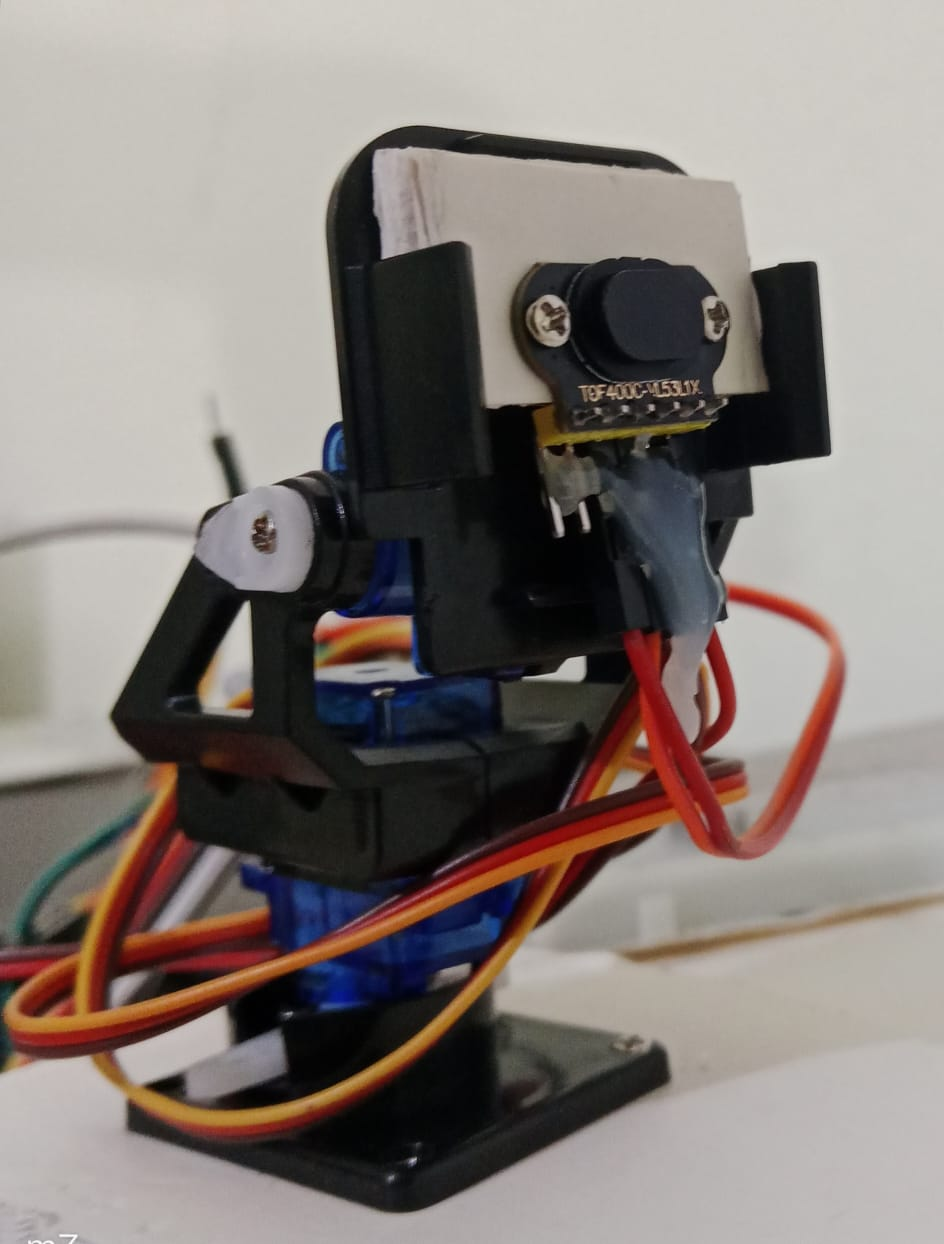
\includegraphics[height=4cm, keepaspectratio]{figures/hardware_setup.png} \\[0.2cm]
                }{}
            }
            {\scriptsize \textcolor{charcoal}{Preliminary SG90-based prototype used for pilot data collection}}
        \end{center}
        \column{0.5\textwidth}
        \begin{center}
            {\Huge \bfseries \textcolor{accent}{68,000+}} \\[0.3cm]
            {\large pilot measurements} \\[0.5cm]
            {\large 2 indoor campaigns} \\[1cm]
            \textcolor{charcoal}{\footnotesize \textbf{\textit{Pilot prototype $\neq$ Final thesis platform}}}
        \end{center}
    \end{columns}
\end{frame}

% SLIDE 9: Scan -> Measure
\begin{frame}{Scan $\rightarrow$ Measure $\rightarrow$ Repeat $\rightarrow$ Reconstruct}
    \begin{center}
        \vspace{0.5cm}
        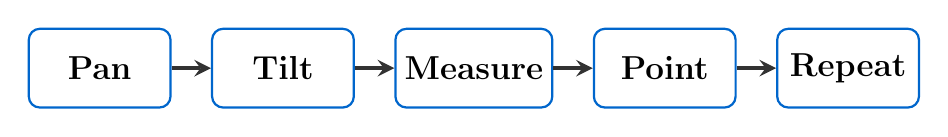
\begin{tikzpicture}[
            box/.style={draw=accent, thick, rounded corners, minimum width=1.8cm, minimum height=1cm, align=center, font=\large\bfseries},
            arrow/.style={->, >=stealth, ultra thick, charcoal}
        ]
            \node[box] (pan) {Pan};
            \node[box, right=0.5cm of pan] (tilt) {Tilt};
            \node[box, right=0.5cm of tilt] (measure) {Measure};
            \node[box, right=0.5cm of measure] (point) {Point};
            \node[box, right=0.5cm of point] (repeat) {Repeat};
            
            \draw[arrow] (pan) -- (tilt);
            \draw[arrow] (tilt) -- (measure);
            \draw[arrow] (measure) -- (point);
            \draw[arrow] (point) -- (repeat);
        \end{tikzpicture}
        
        \vspace{1.5cm}
        {\Large \bfseries \textcolor{navy}{Hundreds of points $\rightarrow$ 3D room}} \\[0.5cm]
        {\large \textcolor{charcoal}{Each distance measurement becomes one 3D point.}}
    \end{center}
\end{frame}

% SLIDE 10: Scale the Evidence
\begin{frame}{Scale the Evidence}
    \begin{center}
        \vspace{0.5cm}
        {\Huge \bfseries \textcolor{accent}{150,000+}} \\[0.3cm]
        {\large measurements} \\[0.5cm]
        
        \begin{columns}
            \column{0.2\textwidth}\centering \IfFileExists{figures/slide9_img0.png}{
\includegraphics[height=1cm]{figures/slide9_img0.png}\\[0.1cm]}{} Indoor
            \column{0.2\textwidth}\centering \IfFileExists{figures/slide9_img1.png}{
\includegraphics[height=1cm]{figures/slide9_img1.png}\\[0.1cm]}{} Outdoor
            \column{0.2\textwidth}\centering \IfFileExists{figures/slide9_img2.png}{
\includegraphics[height=1cm]{figures/slide9_img2.png}\\[0.1cm]}{} Diff. Lighting
            \column{0.2\textwidth}\centering \IfFileExists{figures/slide9_img3.png}{
\includegraphics[height=1cm]{figures/slide9_img3.png}\\[0.1cm]}{} Diff. Surfaces
            \column{0.2\textwidth}\centering \IfFileExists{figures/slide9_img4.png}{
\includegraphics[height=1cm]{figures/slide9_img4.png}\\[0.1cm]}{} Ground Truth
        \end{columns}
        
        \vspace{0.8cm}
        \textcolor{successgreen}{\large \textbf{PROPOSED TARGET: One Unified Dataset}}
    \end{center}
\end{frame}

% SLIDE 11: Will It Work
\begin{frame}{Will It Work in a New Environment?}
    \begin{center}
        \vspace{0.2cm}
        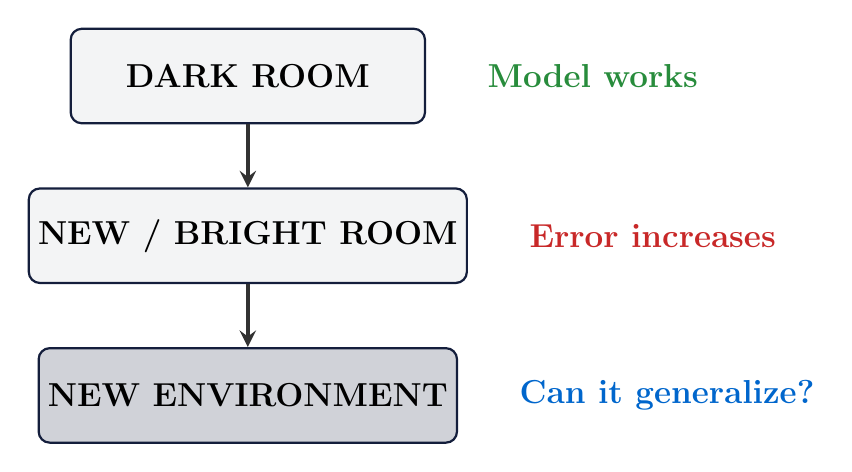
\begin{tikzpicture}[
            box/.style={draw=navy, thick, fill=navy!5, rounded corners, minimum width=4.5cm, minimum height=1.2cm, align=center, font=\large\bfseries}
        ]
            \node[box] (dark) {DARK ROOM};
            \node[right=0.5cm of dark, text=successgreen, font=\large\bfseries] (check) {\IfFileExists{figures/slide10_img1.png}{\raisebox{-0.2cm}{\includegraphics[height=0.8cm]{figures/slide10_img1.png}}}{} Model works};
            
            \node[box, below=0.8cm of dark] (bright) {NEW / BRIGHT ROOM};
            \node[right=0.5cm of bright, text=errorred, font=\large\bfseries] (cross) {\IfFileExists{figures/slide10_img2.png}{\raisebox{-0.2cm}{\includegraphics[height=0.8cm]{figures/slide10_img2.png}}}{} Error increases};
            
            \node[box, fill=navy!20, below=0.8cm of bright] (new) {NEW ENVIRONMENT};
            \node[right=0.5cm of new, text=accent, font=\large\bfseries] (question) {\IfFileExists{figures/slide10_img3.png}{\raisebox{-0.2cm}{\includegraphics[height=0.8cm]{figures/slide10_img3.png}}}{} Can it generalize?};
            
            \draw[->, >=stealth, ultra thick, charcoal] (dark) -- (bright);
            \draw[->, >=stealth, ultra thick, charcoal] (bright) -- (new);
            
            \node[left=0.2cm of dark] {\IfFileExists{figures/slide10_img0.png}{\includegraphics[height=1cm]{figures/slide10_img0.png}}{}};
        \end{tikzpicture}
    \end{center}
\end{frame}

% SLIDE 12: Don't Use Distance Alone
\begin{frame}{Don't Use Distance Alone}
    \begin{center}
        \vspace{0.2cm}
        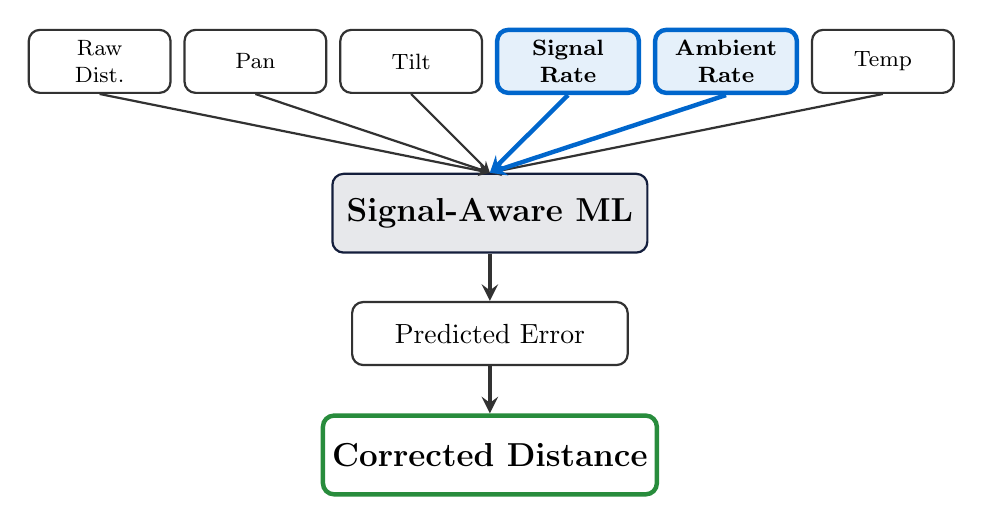
\begin{tikzpicture}[
            feat/.style={draw=charcoal, thick, rounded corners, minimum height=0.8cm, minimum width=1.8cm, align=center, font=\footnotesize},
            highlight/.style={draw=accent, ultra thick, fill=accent!10, rounded corners, minimum height=0.8cm, minimum width=1.8cm, align=center, font=\footnotesize\bfseries}
        ]
            \node[feat] (raw) {Raw\\Dist.};
            \node[feat, right=0.15cm of raw] (pan) {Pan};
            \node[feat, right=0.15cm of pan] (tilt) {Tilt};
            \node[highlight, right=0.15cm of tilt] (sig) {Signal\\Rate};
            \node[highlight, right=0.15cm of sig] (amb) {Ambient\\Rate};
            \node[feat, right=0.15cm of amb] (temp) {Temp};
            
            \node[draw=navy, thick, fill=navy!10, minimum width=4cm, minimum height=1cm, rounded corners, font=\large\bfseries, below=1cm of tilt, xshift=1cm] (ml) {Signal-Aware ML};
            \node[draw=charcoal, thick, minimum width=3.5cm, minimum height=0.8cm, rounded corners, font=\normalsize, below=0.6cm of ml] (err) {Predicted Error};
            \node[draw=successgreen, ultra thick, minimum width=4cm, minimum height=1cm, rounded corners, font=\large\bfseries, below=0.6cm of err] (corr) {Corrected Distance};
            
            \draw[->, >=stealth, thick, charcoal] (raw.south) -- (ml.north);
            \draw[->, >=stealth, thick, charcoal] (pan.south) -- (ml.north);
            \draw[->, >=stealth, thick, charcoal] (tilt.south) -- (ml.north);
            \draw[->, >=stealth, thick, charcoal] (temp.south) -- (ml.north);
            \draw[->, >=stealth, ultra thick, accent] (sig.south) -- (ml.north);
            \draw[->, >=stealth, ultra thick, accent] (amb.south) -- (ml.north);
            \draw[->, >=stealth, ultra thick, charcoal] (ml.south) -- (err.north);
            \draw[->, >=stealth, ultra thick, charcoal] (err.south) -- (corr.north);
        \end{tikzpicture}
    \end{center}
\end{frame}

% SLIDE 13: Python to ESP32
\begin{frame}{From Python to ESP32}
    \begin{center}
        \vspace{0.5cm}
        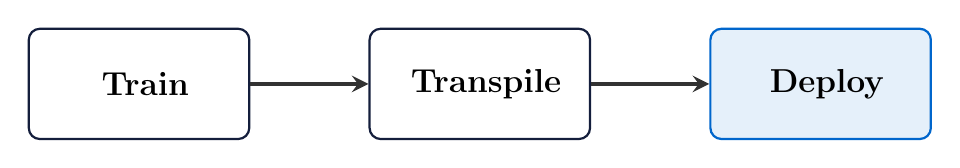
\begin{tikzpicture}[
            node distance=1.5cm,
            box/.style={draw=navy, thick, rounded corners, minimum width=2.8cm, minimum height=1.4cm, align=center, font=\large\bfseries},
            arrow/.style={->, >=stealth, ultra thick, charcoal}
        ]
            \node[box] (train) {\IfFileExists{figures/slide13_img0.png}{\includegraphics[height=0.8cm]{figures/slide13_img0.png}\\[0.1cm]}{} Train};
            \node[box, right=of train] (transpile) {\IfFileExists{figures/slide13_img1.png}{\includegraphics[height=0.8cm]{figures/slide13_img1.png}\\[0.1cm]}{} Transpile};
            \node[box, draw=accent, fill=accent!10, right=of transpile] (deploy) {\IfFileExists{figures/slide13_img2.png}{\includegraphics[height=0.8cm]{figures/slide13_img2.png}\\[0.1cm]}{} Deploy};
            
            \draw[arrow] (train) -- (transpile);
            \draw[arrow] (transpile) -- (deploy);
        \end{tikzpicture}
        
        \vspace{1cm}
        {\Huge \bfseries \textcolor{accent}{$<$ 100 $\mu$s}} \\[0.2cm]
        {\large inference target} \\[0.3cm]
        {\large \textcolor{charcoal}{Zero external runtime dependency}}
    \end{center}
\end{frame}

% SLIDE 14: Pilot Results & Constraints
\begin{frame}{Pilot Results \& Constraints}
    \vspace{0.2cm}
    \begin{columns}[t]
        \column{0.45\textwidth}
        \begin{center}
            {\large \bfseries Pilot Results} \\[0.2cm]
            {\Huge \bfseries \textcolor{successgreen}{94.7\%}} \\[0.1cm]
            {\footnotesize MAE reduction (Day 2)} \\[0.3cm]
            {\Huge \bfseries \textcolor{accent}{22.4 mm}} \\[0.1cm]
            {\footnotesize MAE (pooled training)}
        \end{center}
        
        \column{0.55\textwidth}
        \begin{center}
            {\large \bfseries Limitations \& Constraints} \\[0.2cm]
            \begin{itemize}
                \footnotesize
                \item \textbf{Compute:} ESP32 limits model depth (520KB SRAM).
                \item \textbf{Ground Truth:} Manual ray-plane setup lacks reference LiDAR accuracy.
                \item \textbf{Jitter:} N20/DC motors cause actuation vibration.
            \end{itemize}
        \end{center}
    \end{columns}
\end{frame}

% SLIDE 15: Project Planning
\begin{frame}{Project Planning: Work Division, Budget, \& Timeline}
    \vspace{0.1cm}
    \begin{columns}[t]
        \column{0.45\textwidth}
        \textbf{Timeline (6 Months)}
        \begin{itemize}
            \footnotesize
            \item \textbf{M1:} Hardware Assembly
            \item \textbf{M2:} Ground Truth Calibration
            \item \textbf{M3:} 150K Data Collection
            \item \textbf{M4:} ML Training \& Validation
            \item \textbf{M5:} ESP32 Deployment
            \item \textbf{M6:} Defense \& Thesis
        \end{itemize}
        
        \vspace{0.2cm}
        \textbf{Cost-Benefit Analysis}
        \begin{itemize}
            \footnotesize
            \item \textbf{BoM:} VL53L1X (\$6), ESP32 (\$4), Motors (\$2.4), Sensors (\$5). \textbf{Total: $<$ \$22}
            \item \textbf{Benefit:} Viable 3D sensing at a fraction of commercial \$500+ LiDARs.
        \end{itemize}
        
        \column{0.55\textwidth}
        \textbf{Work Division}
        \begin{itemize}
            \footnotesize
            \item \textbf{Abdul Momit Talukder:} Hardware design, motor actuation, ESP32 firmware.
            \item \textbf{Oishi Farzana:} Data collection, ground truth methodology, dataset prep.
            \item \textbf{Mahfuz Ahmad:} ML training, C-code transpilation, point cloud vis.
        \end{itemize}
    \end{columns}
\end{frame}

% SLIDE 16: Complex Engineering Mapping
\begin{frame}{Complex Engineering Problem \& Activity Mapping}
    \begin{center}
        \textbf{Table 1: Mapping with Complex Engineering Problem solving} \\[0.2cm]
        \resizebox{\textwidth}{!}{%
        \begin{tabular}{|c|c|c|c|c|c|c|}
        \hline
        \textbf{\shortstack{WP1 \\ Depth of \\ Knowledge}} & 
        \textbf{\shortstack{WP2 \\ Range of \\ Conflicting \\ Requirements}} & 
        \textbf{\shortstack{WP3 \\ Depth of \\ Analysis}} & 
        \textbf{\shortstack{WP4 \\ Familiarity of \\ Issues}} & 
        \textbf{\shortstack{WP5 \\ Extent of \\ Applicable \\ Codes}} & 
        \textbf{\shortstack{WP6 \\ Extent of \\ Stakeholder \\ Involvement}} & 
        \textbf{\shortstack{WP7 \\ Interdependence}} \\
        \hline
        \huge \textcolor{accent}{\ding{51}} & \huge \textcolor{accent}{\ding{51}} & \huge \textcolor{accent}{\ding{51}} & \huge \textcolor{accent}{\ding{51}} & & & \\
        \hline
        \end{tabular}}
        
        \vspace{0.6cm}
        \textbf{Table 2: Mapping with complex engineering activities} \\[0.2cm]
        \resizebox{0.8\textwidth}{!}{%
        \begin{tabular}{|c|c|c|c|c|}
        \hline
        \textbf{\shortstack{EA1 \\ Range of \\ resources}} & 
        \textbf{\shortstack{EA2 \\ Level of \\ Interaction}} & 
        \textbf{\shortstack{EA3 \\ Innovation}} & 
        \textbf{\shortstack{EA4 \\ Consequences for society \\ and environment}} & 
        \textbf{\shortstack{EA5 \\ Familiarity}} \\
        \hline
        \huge \textcolor{accent}{\ding{51}} & \huge \textcolor{accent}{\ding{51}} & & & \\
        \hline
        \end{tabular}}
    \end{center}
\end{frame}

% SLIDE 17: Green Computing & Democratization
\begin{frame}{Green Computing \& Societal Impact}
    \vspace{0.2cm}
    \begin{columns}[t]
        \column{0.33\textwidth}
        \begin{center}
            \IfFileExists{figures/slide11_img0.png}{
\includegraphics[height=1.2cm]{figures/slide11_img0.png}\\[0.1cm]}{}
            {\large \bfseries \textcolor{accent}{Education}} \\[0.1cm]
            \footnotesize Affordable research
        \end{center}
        \column{0.33\textwidth}
        \begin{center}
            \IfFileExists{figures/slide11_img1.png}{
\includegraphics[height=1.2cm]{figures/slide11_img1.png}\\[0.1cm]}{}
            {\large \bfseries \textcolor{accent}{Robotics}} \\[0.1cm]
            \footnotesize Low-cost mapping
        \end{center}
        \column{0.33\textwidth}
        \begin{center}
            \IfFileExists{figures/slide11_img2.png}{
\includegraphics[height=1.2cm]{figures/slide11_img2.png}\\[0.1cm]}{}
            {\large \bfseries \textcolor{accent}{Assistive Tech}} \\[0.1cm]
            \footnotesize Obstacle sensing
        \end{center}
    \end{columns}
    \vspace{0.3cm}
    \begin{center}
        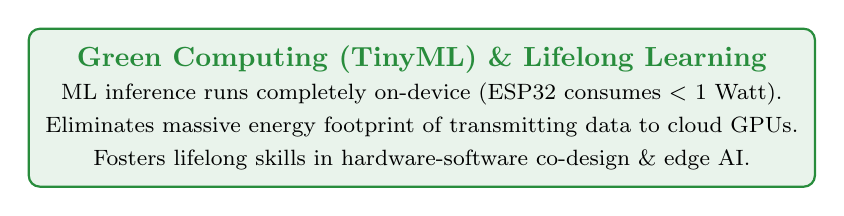
\begin{tikzpicture}
            \node[draw=successgreen, thick, fill=successgreen!10, rounded corners, inner sep=6pt, align=center] {
                \textbf{\textcolor{successgreen}{Green Computing (TinyML) \& Lifelong Learning}} \\
                \footnotesize ML inference runs completely on-device (ESP32 consumes $<$ 1 Watt). \\
                \footnotesize Eliminates massive energy footprint of transmitting data to cloud GPUs.\\
                \footnotesize Fosters lifelong skills in hardware-software co-design \& edge AI.
            };
        \end{tikzpicture}
    \end{center}
\end{frame}

% SLIDE 18: Built to Be Shared & References
\begin{frame}{Built to Be Shared \& References}
    \vspace{0.1cm}
    \begin{columns}[t]
        \column{0.33\textwidth}
        \begin{center}
            \IfFileExists{figures/slide16_img0.png}{
\includegraphics[height=0.8cm]{figures/slide16_img0.png}\\[0.1cm]}{}
            \textbf{\footnotesize CODE (GitHub)}
        \end{center}
        \column{0.33\textwidth}
        \begin{center}
            \IfFileExists{figures/slide16_img1.png}{
\includegraphics[height=0.8cm]{figures/slide16_img1.png}\\[0.1cm]}{}
            \textbf{\footnotesize HARDWARE}
        \end{center}
        \column{0.33\textwidth}
        \begin{center}
            \IfFileExists{figures/slide16_img2.png}{
\includegraphics[height=0.8cm]{figures/slide16_img2.png}\\[0.1cm]}{}
            \textbf{\footnotesize DATASET}
        \end{center}
    \end{columns}
    
    \vspace{0.3cm}
    \textbf{References:}
    \begin{enumerate}
        \footnotesize
        \item A. Corti et al., ``Metrological Characterization of the Kinect V2 ToF,'' \textit{IEEE}, 2016.
        \item H. Su et al., ``DeepToF: Off-the-Shelf Real-Time Correction,'' \textit{ACM}, 2018.
        \item J. Jimenez et al., ``3D scanner based on a ToF camera and a pan-tilt unit,'' \textit{Sensors}, 2014.
    \end{enumerate}
    
    \vspace{0.2cm}
    \begin{center}
        {\Large \bfseries \textcolor{navy}{Thank You. Questions?}}
    \end{center}
\end{frame}

\end{document}
